% Template for URSI Extended Abstracts
%
% Use pdflatex or latex + dvips + ps2pdf to produce a PDF.
%
% 

\documentclass[abstract]{ursi}

%% Add packages and define personal macros here, but ensure that they do not
%% interfere with the fonts and page layout. Do not add hyperlinks.

\title{URSI Extended Abstract Template}

%% Use \affref{nn} and matching \aff{nn}{...} below for several authors
%% Mark the presenting author with an asterisk
\author{First A. Author\affref{ref1}, Second B. Author*\affref{ref1},
  and Third C. Author\affref{ref2}}

%% define affiliations and addresses
\affiliation{%
  % use explicit line-breaks \\ if needed
  \aff{ref1}{ABC University, Prague, Czechia; e-mail: FAA@seznam.cz; SBA@email.cz}
  \aff{ref2}{The Next University, Neverland, USA; e-mail: TCA@gmail.com}
}

% (Omit \affref and \aff and the asterisk if there is only one author.)

\begin{document}

\maketitle

This document describes the obligatory format for URSI Extended Abstracts. The simplest approach is to replace the template’s text with your own. 

The URSI Abstract should be single spaced, single column and \textbf{sized
  for A4 paper} according to this template. The abstract should have a minimum
of approximately \textbf{250 words and be no longer than 1 page} and should be in
English.
%
The body text should be Times New Roman 10~pt., with headings in Times New
Roman 12~pt. The top and bottom, left- and right-hand margins should be
2.5~cm (1~inch). Paragraphs should be separated with one blank line. Do not
indent paragraphs.
%
The title should be centered according to this template. The author's (or
authors') name and complete organizational affiliation should be two lines
below the title. If there are multiple authors, the presenter is to be
identified with an asterisk. The text should start three lines below the
last name.

There should be one section only. It is possible \textbf{(but not required)} to include references, equations, figures, or tables.  Citations and references should follow IEEE format (as used by the 
\emph{Radio Science Bulletin}).  Citations can be of the
form~\cite{cannon,mannix} as is appropriate to the sentence, with the
reference format illustrated at the end of this template.
Equations should be centered with the equation numbers right justified in
the following format:
\begin{equation}
  \label{eq:T}
  T' = \frac{r_\text{e}^2\lambda^2GC_\text{s}L
    \sec\theta\sqrt{\pi}\ \Gamma\!\left(\frac\rho2\right)}
  {4\pi^2\,\Gamma\!\left(\frac{\rho+1}{2}\right)}.
\end{equation}

Figures should include a caption beneath the figure (in Times Roman 10 pt.)
and the caption should include the Figure number in
bold. Figure~\ref{fig:asc} provides an example.
Likewise, tables should include a caption (in Times Roman 10 pt.) but this
time above the table. The caption should include the table number in bold.

\begin{figure}[htbp]
  \centering
  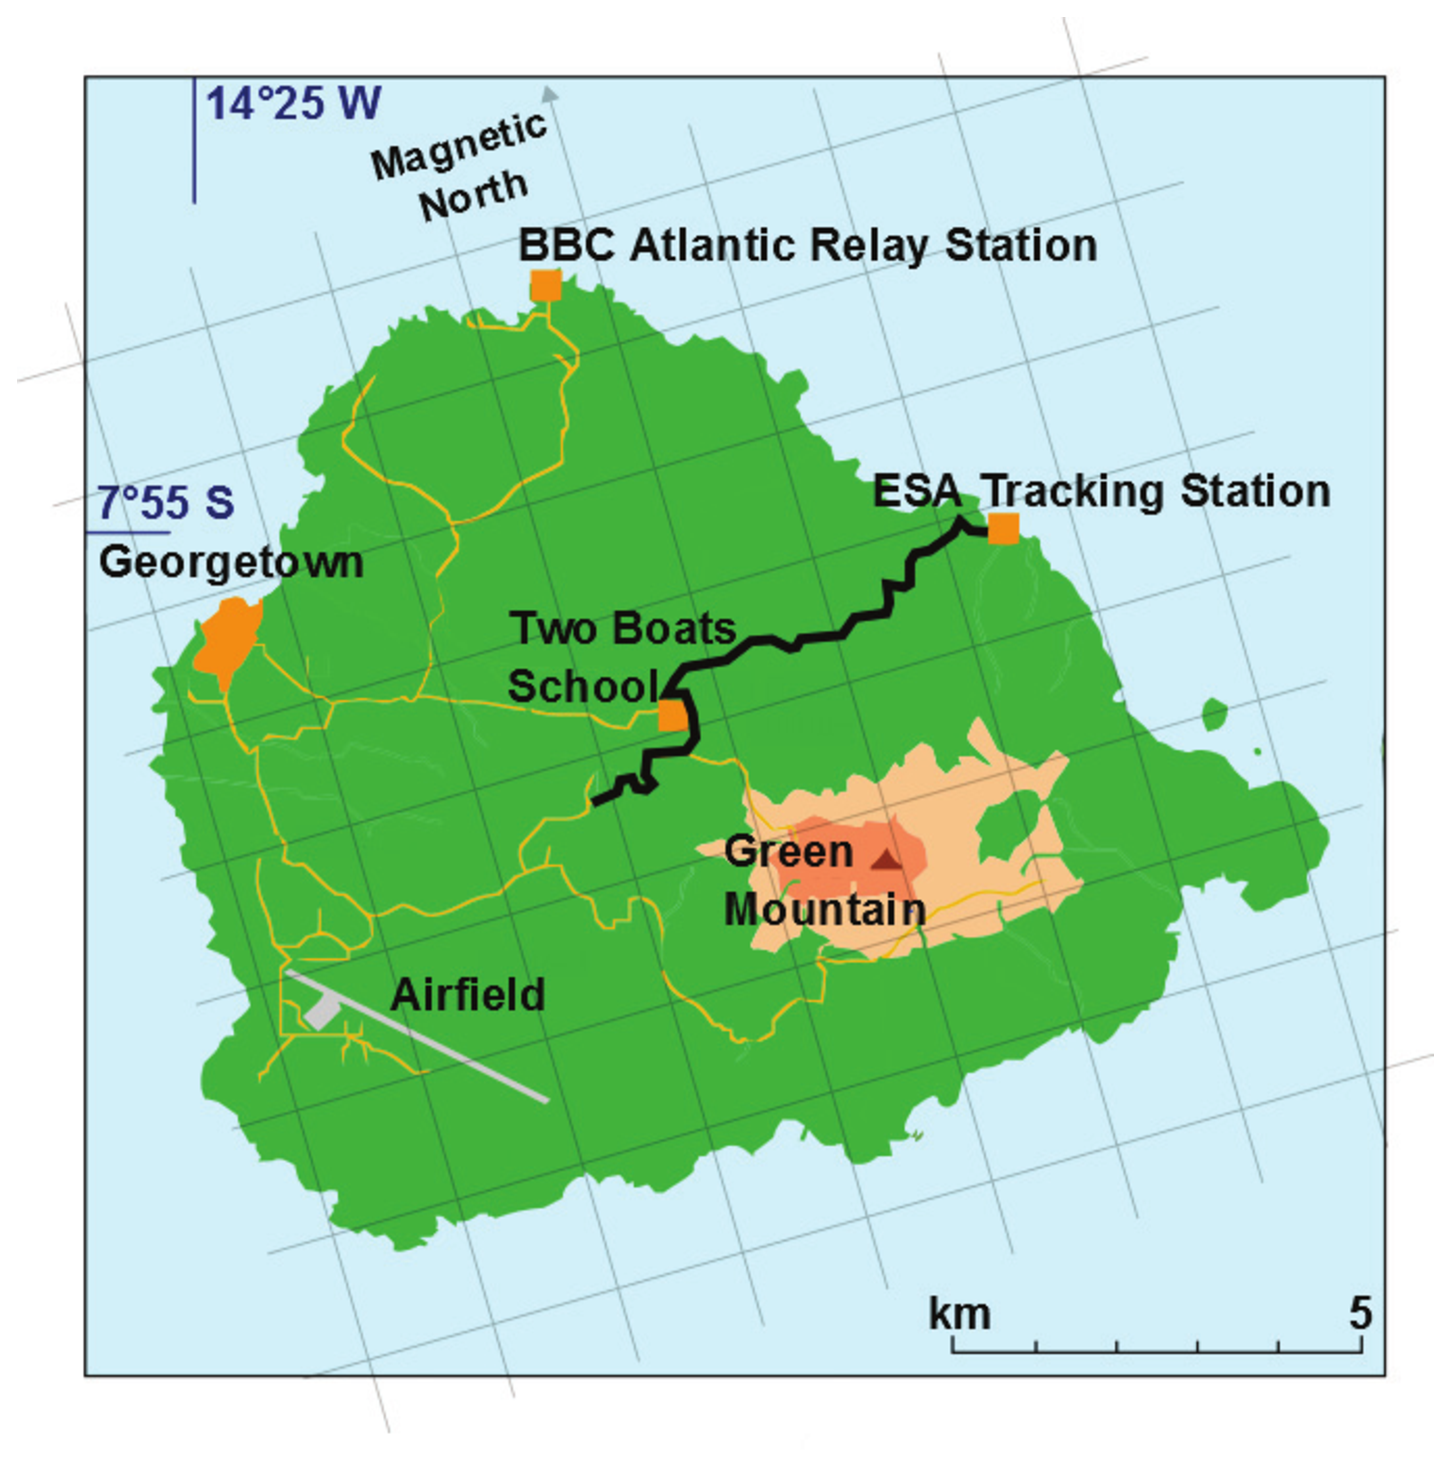
\includegraphics[width=42mm]{ascension_island}
  \caption{Ascension Island (7.9\textdegree S, 14.8\textdegree W showing
    the ESA Tracking Station which was the location of the fixed receiver
    and the road (shown in black) along which the mobile measurements were
    made).}
  \label{fig:asc}
\end{figure}

All submissions will be electronic and in a PDF format (*.pdf) and all
fonts must be embedded in the submitted PDF document.
Embedded Type~1 or True Type fonts are required in the submitted PDF file
as subset fonts. Type~3 fonts (bitmaps) will not be accepted. 

\begin{thebibliography}{99}
\bibitem{cannon} P. S. Cannon, ``Extreme Space Weather --- A Report
  Published by the UK Royal Academy of Engineering,'' \emph{Space Weather},
  \textbf{11}, 4, April 2013, pp. 138--139, doi:10.1002/swe.20032.
\bibitem{mannix} C. R. Mannix, D. P. Belcher, P. S. Cannon, and
  M. J. Angling, ``Using GNSS Signals as a Proxy for SAR Signals:
  Correcting Ionospheric Defocusing,'' \emph{Radio Science}, \textbf{51},
  2, February 2016, pp. 60--70, doi: 10.1002/2015RS005822.
\end{thebibliography}



\end{document}
